% Options for packages loaded elsewhere
\PassOptionsToPackage{unicode}{hyperref}
\PassOptionsToPackage{hyphens}{url}
%
\documentclass[
]{book}
\title{Conception orientée service - Service Oriented Analysis and Design}
\author{Constantin Drabo}
\date{2022-06-17}

\usepackage{amsmath,amssymb}
\usepackage[]{libertine}
\usepackage{iftex}
\ifPDFTeX
  \usepackage[T1]{fontenc}
  \usepackage[utf8]{inputenc}
  \usepackage{textcomp} % provide euro and other symbols
\else % if luatex or xetex
  \usepackage{unicode-math}
  \defaultfontfeatures{Scale=MatchLowercase}
  \defaultfontfeatures[\rmfamily]{Ligatures=TeX,Scale=1}
\fi
% Use upquote if available, for straight quotes in verbatim environments
\IfFileExists{upquote.sty}{\usepackage{upquote}}{}
\IfFileExists{microtype.sty}{% use microtype if available
  \usepackage[]{microtype}
  \UseMicrotypeSet[protrusion]{basicmath} % disable protrusion for tt fonts
}{}
\makeatletter
\@ifundefined{KOMAClassName}{% if non-KOMA class
  \IfFileExists{parskip.sty}{%
    \usepackage{parskip}
  }{% else
    \setlength{\parindent}{0pt}
    \setlength{\parskip}{6pt plus 2pt minus 1pt}}
}{% if KOMA class
  \KOMAoptions{parskip=half}}
\makeatother
\usepackage{xcolor}
\IfFileExists{xurl.sty}{\usepackage{xurl}}{} % add URL line breaks if available
\IfFileExists{bookmark.sty}{\usepackage{bookmark}}{\usepackage{hyperref}}
\hypersetup{
  pdftitle={Conception orientée service - Service Oriented Analysis and Design},
  pdfauthor={Constantin Drabo},
  hidelinks,
  pdfcreator={LaTeX via pandoc}}
\urlstyle{same} % disable monospaced font for URLs
\usepackage[margin=1in]{geometry}
\usepackage{color}
\usepackage{fancyvrb}
\newcommand{\VerbBar}{|}
\newcommand{\VERB}{\Verb[commandchars=\\\{\}]}
\DefineVerbatimEnvironment{Highlighting}{Verbatim}{commandchars=\\\{\}}
% Add ',fontsize=\small' for more characters per line
\usepackage{framed}
\definecolor{shadecolor}{RGB}{248,248,248}
\newenvironment{Shaded}{\begin{snugshade}}{\end{snugshade}}
\newcommand{\AlertTok}[1]{\textcolor[rgb]{0.94,0.16,0.16}{#1}}
\newcommand{\AnnotationTok}[1]{\textcolor[rgb]{0.56,0.35,0.01}{\textbf{\textit{#1}}}}
\newcommand{\AttributeTok}[1]{\textcolor[rgb]{0.77,0.63,0.00}{#1}}
\newcommand{\BaseNTok}[1]{\textcolor[rgb]{0.00,0.00,0.81}{#1}}
\newcommand{\BuiltInTok}[1]{#1}
\newcommand{\CharTok}[1]{\textcolor[rgb]{0.31,0.60,0.02}{#1}}
\newcommand{\CommentTok}[1]{\textcolor[rgb]{0.56,0.35,0.01}{\textit{#1}}}
\newcommand{\CommentVarTok}[1]{\textcolor[rgb]{0.56,0.35,0.01}{\textbf{\textit{#1}}}}
\newcommand{\ConstantTok}[1]{\textcolor[rgb]{0.00,0.00,0.00}{#1}}
\newcommand{\ControlFlowTok}[1]{\textcolor[rgb]{0.13,0.29,0.53}{\textbf{#1}}}
\newcommand{\DataTypeTok}[1]{\textcolor[rgb]{0.13,0.29,0.53}{#1}}
\newcommand{\DecValTok}[1]{\textcolor[rgb]{0.00,0.00,0.81}{#1}}
\newcommand{\DocumentationTok}[1]{\textcolor[rgb]{0.56,0.35,0.01}{\textbf{\textit{#1}}}}
\newcommand{\ErrorTok}[1]{\textcolor[rgb]{0.64,0.00,0.00}{\textbf{#1}}}
\newcommand{\ExtensionTok}[1]{#1}
\newcommand{\FloatTok}[1]{\textcolor[rgb]{0.00,0.00,0.81}{#1}}
\newcommand{\FunctionTok}[1]{\textcolor[rgb]{0.00,0.00,0.00}{#1}}
\newcommand{\ImportTok}[1]{#1}
\newcommand{\InformationTok}[1]{\textcolor[rgb]{0.56,0.35,0.01}{\textbf{\textit{#1}}}}
\newcommand{\KeywordTok}[1]{\textcolor[rgb]{0.13,0.29,0.53}{\textbf{#1}}}
\newcommand{\NormalTok}[1]{#1}
\newcommand{\OperatorTok}[1]{\textcolor[rgb]{0.81,0.36,0.00}{\textbf{#1}}}
\newcommand{\OtherTok}[1]{\textcolor[rgb]{0.56,0.35,0.01}{#1}}
\newcommand{\PreprocessorTok}[1]{\textcolor[rgb]{0.56,0.35,0.01}{\textit{#1}}}
\newcommand{\RegionMarkerTok}[1]{#1}
\newcommand{\SpecialCharTok}[1]{\textcolor[rgb]{0.00,0.00,0.00}{#1}}
\newcommand{\SpecialStringTok}[1]{\textcolor[rgb]{0.31,0.60,0.02}{#1}}
\newcommand{\StringTok}[1]{\textcolor[rgb]{0.31,0.60,0.02}{#1}}
\newcommand{\VariableTok}[1]{\textcolor[rgb]{0.00,0.00,0.00}{#1}}
\newcommand{\VerbatimStringTok}[1]{\textcolor[rgb]{0.31,0.60,0.02}{#1}}
\newcommand{\WarningTok}[1]{\textcolor[rgb]{0.56,0.35,0.01}{\textbf{\textit{#1}}}}
\usepackage{longtable,booktabs,array}
\usepackage{calc} % for calculating minipage widths
% Correct order of tables after \paragraph or \subparagraph
\usepackage{etoolbox}
\makeatletter
\patchcmd\longtable{\par}{\if@noskipsec\mbox{}\fi\par}{}{}
\makeatother
% Allow footnotes in longtable head/foot
\IfFileExists{footnotehyper.sty}{\usepackage{footnotehyper}}{\usepackage{footnote}}
\makesavenoteenv{longtable}
\usepackage{graphicx}
\makeatletter
\def\maxwidth{\ifdim\Gin@nat@width>\linewidth\linewidth\else\Gin@nat@width\fi}
\def\maxheight{\ifdim\Gin@nat@height>\textheight\textheight\else\Gin@nat@height\fi}
\makeatother
% Scale images if necessary, so that they will not overflow the page
% margins by default, and it is still possible to overwrite the defaults
% using explicit options in \includegraphics[width, height, ...]{}
\setkeys{Gin}{width=\maxwidth,height=\maxheight,keepaspectratio}
% Set default figure placement to htbp
\makeatletter
\def\fps@figure{htbp}
\makeatother
\setlength{\emergencystretch}{3em} % prevent overfull lines
\providecommand{\tightlist}{%
  \setlength{\itemsep}{0pt}\setlength{\parskip}{0pt}}
\setcounter{secnumdepth}{5}
\usepackage{booktabs}
\ifLuaTeX
  \usepackage{selnolig}  % disable illegal ligatures
\fi
\usepackage[]{natbib}
\bibliographystyle{apsr}

\usepackage{amsthm}
\newtheorem{theorem}{Theorem}[chapter]
\newtheorem{lemma}{Lemma}[chapter]
\newtheorem{corollary}{Corollary}[chapter]
\newtheorem{proposition}{Proposition}[chapter]
\newtheorem{conjecture}{Conjecture}[chapter]
\theoremstyle{definition}
\newtheorem{definition}{Definition}[chapter]
\theoremstyle{definition}
\newtheorem{example}{Example}[chapter]
\theoremstyle{definition}
\newtheorem{exercise}{Exercise}[chapter]
\theoremstyle{definition}
\newtheorem{hypothesis}{Hypothesis}[chapter]
\theoremstyle{remark}
\newtheorem*{remark}{Remark}
\newtheorem*{solution}{Solution}
\begin{document}
\maketitle

{
\setcounter{tocdepth}{1}
\tableofcontents
}
\hypertarget{les-concepts}{%
\chapter{Les concepts}\label{les-concepts}}

Dans ce chapitre nous allons faire le tour des différents concepts qui entrent dans la compréhension de la conception orientée service. Il s'agira de définir la notion de \textbf{SOAD} (\emph{Service Oriented Analysis and Design}), la définition du \textbf{SOA} (\emph{Service Oriented Application}).

\hypertarget{duxe9finition}{%
\section{Définition}\label{duxe9finition}}

L'analyse et la conception orientée services (\textbf{SOAD} : \emph{Service Oriented Analysis and Design}) est une méthodologie qui fait référence à la modélisation et à la conception d'application d'architecture orientée services (\textbf{SOA}: \emph{Service Oriented Application}). Une approche SOAD dans la conception SOA nécessite les éléments clés suivants:

\begin{itemize}
\tightlist
\item
  \textbf{modèle de processus}
\item
  \textbf{instructions}
\item
  \textbf{normes}
\item
  \textbf{artefacts}
\item
  \textbf{qualité de service}
\end{itemize}

\textbf{Modèle de processus}: elle consiste en la définition du processus et de la notation en faisant un mélange de l'analyse orientée objet (\textbf{OOAD}), la modélisation des processus métier (\textbf{BPM}) et les éléments d'architecture d'entreprise.

\textbf{Instruction}: c'est la manière structurée de conceptualiser les services

\textbf{Normes} : fournir des facteurs de qualité bien définis et les meilleurs pratiques de service, de capacité, de données et de granularité des contraintes. Les rôles doivent être bien définis et indiquer si c'est un développeur, un architect ou un analyste qui est responsable de chaque fraction de travail.

\textbf{Artefacts}: elle consite à définir ce qui n'est pas un bon service, comme les services qui ne sont pas réutilisables, et qui ne sont donc pas considérés comme des résidents SOA.

\textbf{Qualité de service}: elle facilite la modélisation de bout en bout et fournit un support complet d'outils.

\hypertarget{quest-ce-que-la-soa}{%
\section{Qu'est-ce-que la SOA}\label{quest-ce-que-la-soa}}

La \textbf{SOA} (\_Service Oriented Architecture) est un modèle de conception qui rend des composants logiciels réutilisables, grâce à des interfaces de services qui utilisent un langage commun pour communiquer via un réseau.

Un \textbf{service} est une unité autonome de fonctionnalité logicielle, ou d'un ensemble de fonctionnalités, conçue pour réaliser une tâche précise comme récupérer des informations ou exécuter une opération.

Il contient les intégrations de code et de données nécessaires pour exécuter une fonction métier distincte et complète. Vous pouvez y accéder à distance, et interagir avec lui ou le mettre à jour de manière indépendante. En d'autre termes, l'architecture SOA permet à des composants logiciels déployés et gérés séparement de communiquer et de fonctionner ensemble sous la forme d'applications logicielles communes à différents systèmes.

L'approche \textbf{SOA} intègre nativement les principes de \emph{modularité}, d'\emph{interfaçage}, de \emph{contractualisation}, et d'\emph{interopérabilité}. Elle assure ainsi une adaptation rapide du système d'informationn au regard des évolutions des besoins de l'entreprise. Elle permet également de capitaliser la mise en place de bonnes pratiques par l'élaboration d'une architecture de reference. Cette architecture de référence pourra également être utilisée pour répondre à des problématiques de convergence de systèmes.

\begin{center}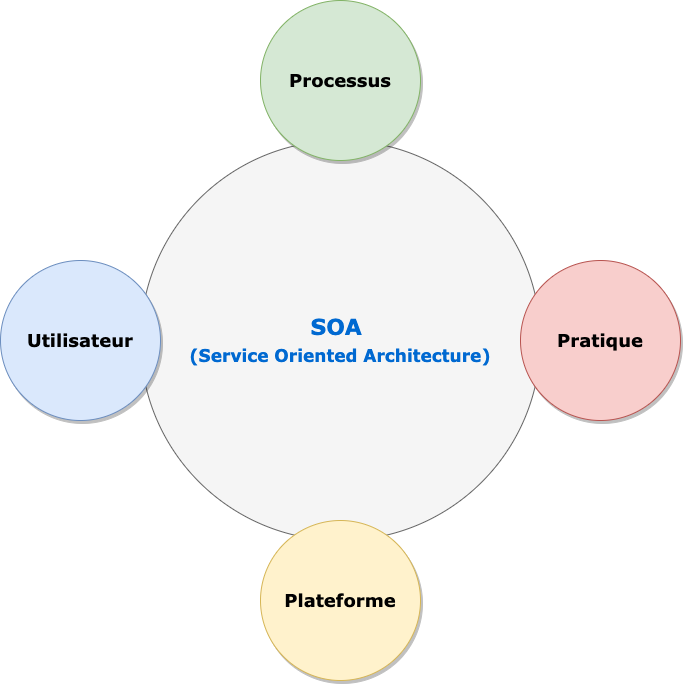
\includegraphics[width=0.7\linewidth]{SOA} \end{center}

L'architecture SOA se base sur ressources de l'entreprise pour fournir un système informatique efficient.

\begin{itemize}
\tightlist
\item
  \emph{Pratique} : elle utilise les best-practices de l'entreprise pour construire une architecture efficace
\item
  \emph{Plateforme} : augmenter l'efficacité opérationnelle
\item
  \emph{Utilisateur} : elle donne aux utilisateurs le pouvoir de prendre de meilleures décisions
\item
  \emph{Processus} : aligner l'IT au processus métiers de l'entreprise
\end{itemize}

Selon le \textbf{Gartner Group Research}, une application qui obéit à la SOA doit respecter les cinq(5) principes suivants:

\begin{enumerate}
\def\labelenumi{\arabic{enumi}.}
\tightlist
\item
  \emph{le système doit être modulaire}. Cela offre l'avantage évident de pouvoir diviser et régner (résoudre un problème complexe en assemblant un ensemble de petits composants simples qui fonctionnent ensemble)
\item
  \emph{les modules doivent être distribuables}. Ils doivent être capables de fonctionner sur des ordinateurs différents et communiquent entre eux en envoyant des messages sur un réseau lors de leur exécution.
\item
  \emph{les interfaces d'un module doivent être clairement définies et documentées}. Les développeurs de logiciels écrivent ou génèrent des métadonnées d'interface qui spécifient un contrat explicite afin qu'un autre développeur puisse trouver et utiliser le service (cela permet un couplage faible)
\item
  \emph{un module qui implémente un service peut être remplacé par un autre module qui offre le même service et la même interface}, car l'interface conçue est distincte du module. Il s'agit d'un aspect du couplage faible qui permet une maintenance et des améliorations continues.
\item
  \emph{les modules du fournisseur de services doivent être partageables}. Ils sont conçus et déployés de manière à pouvoir être invoqués successivement par des modules consommateurs de services disparates engagés dans des activités métiers diverses, bien que partiellement liées.
  \#\#\# Comment fonctionne l'architecture orientée service
\end{enumerate}

Pour implémenter l'architecture orientée service (\textbf{SOA}) il existe une panoplie de technologies disponibles. Le choix technologique dépend du besoin de chaque entreprise. En général, une architecture orientée service utilise les services web pour son implémentation. Les services web sont une technologie qui permet de rendre les blocs fonctionnels accessibles à travers Internet. Parmi les possibilités de web service, nous avons l'implémentation du standard \textbf{SOAP} (\emph{Simple Object Access Protocol}) , l'utilisation de l'architecture \textbf{REST} (\emph{Representational State Transfer}). Il est également possible d'utiliser des technologies basées sur l'échange de message telle que \textbf{ActiveMQ}, \textbf{Apache ActiveMQ Artemis}, \textbf{Kafka}, etc. Les déveoppeurs peuvent également utiliser des modèles appelés \textbf{ESB} (\emph{Enterprise Service Bus}) pour réaliser l'intégration entre unn composant centralisé et les systèmes backe-end, puis les rendre disponibles en tant qu'interfaces de services.

\hypertarget{soa-vs-approche-monolithique}{%
\subsection{SOA vs approche monolithique}\label{soa-vs-approche-monolithique}}

Il existe plusieurs avantages à l'architecture orientée service spécialement pour un service web basé métier. Dans les lignes qui suivront, nous allons exposer quelques unes de ces bénéfices.

\underline{Utiliser une architecture orientée service pour créer un code réutilisable} : Non seulement cela réduit le temps consacré au processus de développement, mais il n'y a aucune raison de réinventer la roue de codage chaque fois que vous devez créer un nouveau service ou processus. L'architecture orientée services permet également d'utiliser plusieurs langages de codage car tout passe par une interface centrale.

\underline{Utiliser une architecture orientée service pour promouvoir l'interaction} : Avec l'architecture orientée services, une forme standard de communication est mise en place, permettant aux différents systèmes et plates-formes de fonctionner indépendamment les uns des autres. Grâce à cette interaction, l'architecture orientée services est également capable de contourner les pare-feu, permettant « aux entreprises de partager des services vitaux pour les opérations ».

\underline{Utiliser une architecture orientée service pour la scalabilité} : Il est important de pouvoir faire évoluer une entreprise pour répondre aux besoins du client, mais certaines dépendances peuvent entraver cette évolutivité. L'utilisation de l'architecture orientée services réduit l'interaction client-service, ce qui permet une plus grande évolutivité.

\underline{Utiliser une architecture orientée service les coûts} : Avec l'architecture orientée services, il est possible de réduire les coûts tout en « maintenant un niveau de sortie souhaité ». L'utilisation de l'architecture orientée services permet aux entreprises de limiter la quantité d'analyses requises lors du développement de solutions personnalisées.

\begin{center}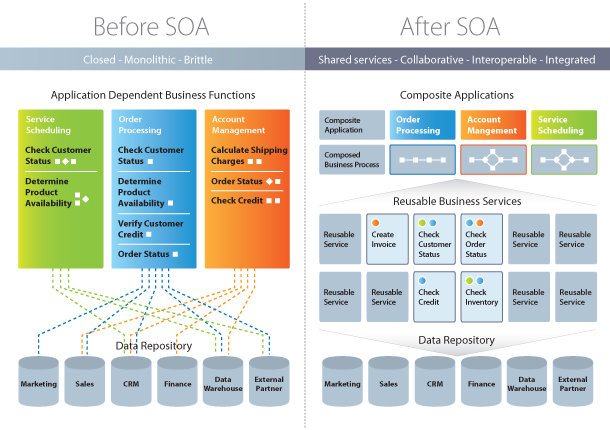
\includegraphics[width=0.7\linewidth]{soavsmono} \end{center}

\hypertarget{les-ruxf4les-au-sein-dune-architecture-orientuxe9e-service-soa}{%
\subsection{Les rôles au sein d'une architecture orientée service (SOA)}\label{les-ruxf4les-au-sein-dune-architecture-orientuxe9e-service-soa}}

Trois (3) rôles fournissent les principaux composants d'une architecture orientée service :

\begin{itemize}
\tightlist
\item
  le fournisseur de service
\item
  le broker ou registre de service
\item
  le demandeur ou consommateur de service
\end{itemize}

\textbf{Fournisseur ou producteur} : un fournisseur crée des services web qu'il met à la disposition dans un \textbf{registre de services}. Il est responsable des conditions d'utilisation de ces services.

\textbf{Broker ou registre de service} : un borker ou registre de services est chargé de fournir les informations sur le service au \textbf{demandeur}. Le broker peut être public ou privé.

\textbf{Demandeur ou consommateur} : le consommateur de services cherche un service dans un broker ou registre de services, puis se connecte à un \textbf{fournisseur de service} pour obtenir le service en question.

\begin{center}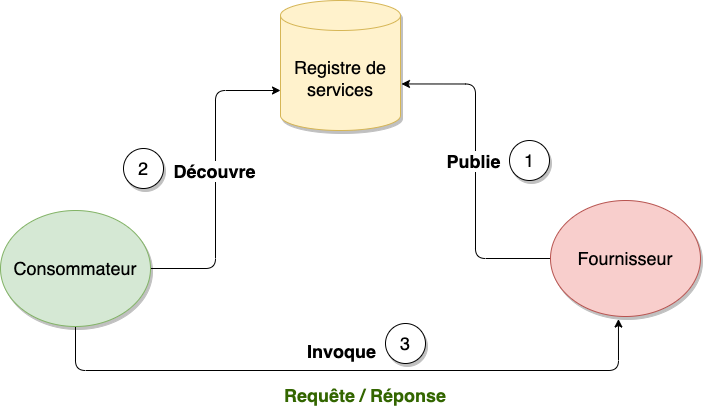
\includegraphics[width=0.7\linewidth]{roles} \end{center}

\hypertarget{les-extensions-de-larchitecture-soa---architecture-uxe9venementielle-event-driven-architecture}{%
\subsection{Les extensions de l'architecture SOA - Architecture évenementielle (Event-Driven Architecture)}\label{les-extensions-de-larchitecture-soa---architecture-uxe9venementielle-event-driven-architecture}}

Dans un système orienté événements, la structure centrale de la solution repose sur la capture, la communication, le traitement et la persistence des événements. C'est ce qui différencie ce type de système du modèle traditionnel orienté requête.

\textbf{Evénement} : un événement désigne tout phénomène ou changement d'état significatif au niveau du matériel ou d'un logiciel système. Il ne faut pas confondre un événemet et une notification d'évenement, c'est-à-dire une notification ou un message envoyé par le système pour signaler à une autre partie du système qu'un événement s'est produit.
Les événements peuvent être causés par des actions internes ou externes. Ils peuvent être provoqués par des utilisateurs ( clics de souris ou frappe sur le clavier, par exemple), provenir d'une source externe (un capteur) ou être générés par le système (lors du chargement d'un programme, par exemple).

Ce type d'architecture implique des \textbf{producteurs} et des \textbf{consommateurs} d'événements. Un producteur d'événements détecte ou reconnaît un événement et le représente sous forme de message. Il ignore quels seront les consommateurs et les conséquences de chaque événement.
Lorsqu'un évenement a été détecté, il est transmis du producteur au consommateur via des \textbf{canaux d'événement}, où une plateforme de traitemennt les prend en charge de façon asynchrone. Les consommateurs doivent être informés lorsqu'un événement se produit. Ils peuvent traiter l'événement ou être seulement affectés par ce dernier.
La plateforme de traitement des événements exécute ma reponse adaptée à chaque événement et envoie l'activité en aval au consommateurs concernés. Cette activité permet de visualiser le résultat d'un événement.

Une architecture orientée événements peut être basée sur un modèle de \textbf{publication/abonnement} ou sur un modèle de \textbf{flux d'événements} .

\begin{itemize}
\item
  le modèle de \textbf{publication/abonnement} : ce modèle est une infrastructure de messagerie basée sur des abonnements à flux d'événements. Lorsqu'il est utilisé, chaque fois qu'un événement se produit ou est publié, il est envoyé aux abonnés qui doivent en être informés.
\item
  le modèle de \textbf{flux d'événement} : avec ce modèle de flux d'événements, les évenements sont enregistrés dans un journal. Au lieu d'être abonnés à un flux d'évenements, les consommateurs peuvent accéder à n'importe quelle partie du flux et le rejoindre à tout moment.
\end{itemize}

\hypertarget{les-extensions-de-larchitecture-soa---les-api-application-programming-interface}{%
\subsection{Les extensions de l'architecture SOA - Les API (Application Programming Interface)}\label{les-extensions-de-larchitecture-soa---les-api-application-programming-interface}}

Une \textbf{API} ou \textbf{Interface de Programmation d'Application}, est un ensemble de définitions et de protocoles qui facilite la création et l'intégration de logiciel d'applications.
Les API permettent à votre produit ou service de communiquer avec d'autres produits et services sans connaître les détails de leur implémentation.
Les API sont parfois considérés comme des contrats avec une documentation qui constitue un accord entre les parties : si la \textbf{partie 1} envoie une requête à distance selon une structure particulière, le logiciel de la \textbf{partie 2} devra répondre selon les conditions définies.

\begin{center}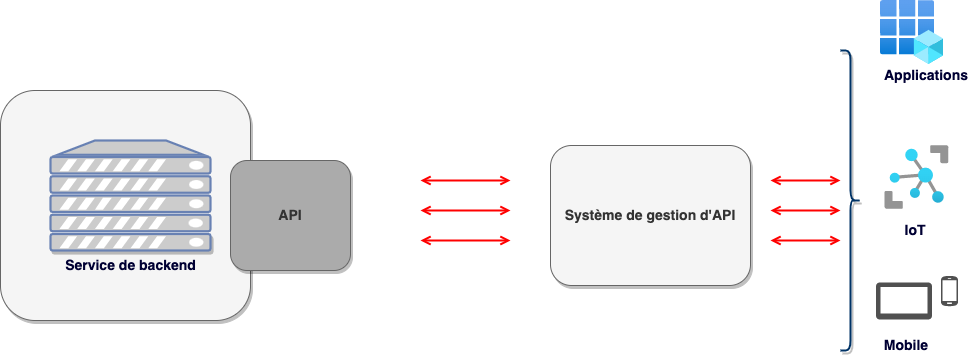
\includegraphics[width=0.7\linewidth]{api} \end{center}

Il existe plusieurs type d'API : les \textbf{API privées} , les \textbf{API publiques} et les \textbf{API partenaires}.

L'\textbf{API privée} est utilisables qu'en interne de l'entreprise. Cette approche permet d'avoir un contrôle total sur l'API.

L'\textbf{API publique} est accessible à tous. Cette approche autorise les tiers à développer des applications qui interagissent avec votre API et peut devenir source d'innovations.

L'\textbf{API partenaire} est partagée avec certains partenaires de l'entreprise. Cette approche peut générer de nouveaux flux de revenus sans compromettre la sécurité.

\hypertarget{les-extensions-de-larchitecture-soa---les-microservices}{%
\subsection{Les extensions de l'architecture SOA - Les microservices}\label{les-extensions-de-larchitecture-soa---les-microservices}}

Les \textbf{microservices} sont une interprétation moderne des architectures orientées services utilisées pour créer des systèmes logiciels distribués. Ils ont une nouvelle approche de réalisation et de mise en oeuvre de la SOA qui met l'accent également sur le déploiement continu et d'autres pratiques agiles (\textbf{DevOps}).

Les architectures de microservices fonctionnent d'une manière très similaires à la SOA, dans le sens où elles utilisent des services faiblement couplés. Par contre, elles poussent la destructuration de l'architecture classique encore plus loin.

Les services qui compose l'architecture de microservices utilisent une structure de messagerie commune, telle que le \textbf{API RESTful}. Ils se servent des API RESTful pour communiquer entre eux simplement sans convertir leurs données ni recourir à des couches d'intégration supplémentaires. L'utilisation des API RESTful permet et favorise même l'accélération de la distribution es nouvelles fonctions et mises à jour.

Chaque service est distinct. Vous pouvez remplacer, améliorer ou supprimer chacun d'entre eux sans affecter les autres services de l'architecture. Cette architecture légère vous aide à optimiser les ressources distribuées ou Cloud et à faire évoluer chaque service de façon dynamique.

Les égalements ci-après caractérisent les microservices :

\begin{itemize}
\item
  des interfaces fines (vers des services déployables indépendamment)
\item
  développement axé sur les affaires ( par exemple, conception axée sur le domaine)
\item
  architectures applicatives cloud
\item
  programmation polyglotte et persistence
\item
  déploiement de conteneurs légers
\item
  livraison continue décentralisée
\item
  DevOps avec une surveillance holistique des services.
\end{itemize}

\hypertarget{preview-book}{%
\section{Preview book}\label{preview-book}}

As you work, you may start a local server to live preview this HTML book. This preview will update as you edit the book when you save individual .Rmd files. You can start the server in a work session by using the RStudio add-in ``Preview book'', or from the R console:

\begin{Shaded}
\begin{Highlighting}[]
\NormalTok{bookdown}\SpecialCharTok{::}\FunctionTok{serve\_book}\NormalTok{()}
\end{Highlighting}
\end{Shaded}

\hypertarget{moduxe8le-de-cycle-de-vie}{%
\chapter{Modèle de cycle de vie}\label{moduxe8le-de-cycle-de-vie}}

Ce chapitre va aborder le cycle de développement et le cycle de vie des applications orienté service.

Un service est quelque chose qui nait à un certain moment pour accomplir une tache précise qui peut s'achever ou pas. Un service est une entité qui vit pour une certaine raison, peut durer un certain temps et peut ou non être retiré en raison des circonstances.

Un service est une matérialisation de solution logicielle qui est créée dans le but de résoudre un problème commercial ou technologique, mais qui est également un élément de mise en œuvre qui doit coexister avec d'autres actifs logiciels.

Dans la suite du document, nous allons faire ressortir les préoccupations organisationelles des entreprises, façonnées par la discipline de modélisation de la SOA et allons terminer par l'implémentation de la solution informatisée.

Il n'y a rien de \textbf{cyclique} dans le cycle de vie des services, et même si nous le souhaitons, les services ne durent pas éternellement. Alors que les services continuent d'évoluer et d'apporter de la valeur à leurs consommateurs et contribuent de manière significative dans les environnement de production au sein des entrerprises, ils sont toujours sujets à la perfection et aux amélioration. Cela nécessite généralement une investigation pour déterminer si un service doit être ramener à la forge de conception pour une refaire l'architecture ou initier une reconstruction. Ce processus répétitif est appelé le cycle de vie du service.
La figure ci-dessous illustre le cycle de vie d'un service :

\begin{center}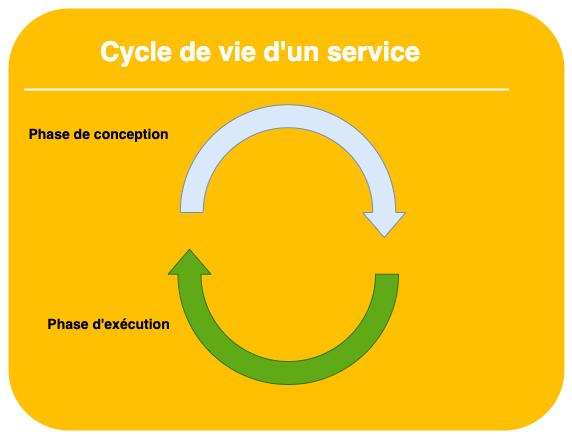
\includegraphics[width=0.7\linewidth]{cyclevie} \end{center}

\hypertarget{principe-du-moduxe8le-de-cycle-de-vie-orientuxe9-service}{%
\section{Principe du modèle de cycle de vie orienté service}\label{principe-du-moduxe8le-de-cycle-de-vie-orientuxe9-service}}

Les principes du cycle de vie d'un service sont les bonnes pratiques rudimentaires pour instituer une méthodologie du cycle de vie d'une SOA afin de gérer les initiatives métiers d'une organisation et le processus de développement d'un service. Ils abordent les fondamentaux de la gestion des frameworks, la planification, les préoccupations structurelles en rapport avec les sujets suivants :
la métamorphose du service, la stratégie, la gouvernance, la structure, le financement, le retour sur investissement (ROI).

Le modèle du cycle de vie de la SOA est basé sur le \textbf{\emph{principe de la stratégie}} qui a un impact sur tous les aspects du cycle de vie du service, telles que la planification d'initiatives de cycle de vie et la fourniture d'une feuille de route détaillée. Le \textbf{\emph{principe de la gouvernance}} se focalise sur les bonnes pratiques de l'orienté service et les standards pour faciliter la gestion et l'exécution du cycle de vie pour superviser les activités. le \textbf{\emph{principe de structure}} développe les éléments du cadre du cycle de vie. Le système de \textbf{\emph{financement}} du projet est un autre important principe qui introduit un nouveau regard sur le développement des services et la budgétisation des opérations. Le \textbf{\emph{principe du retour sur investissement}} met l'accent sur l'importance du suivi des revenus générés par les opérations de service. Enfin, le \textbf{\emph{principe de métamorphose}}, qui incarne la stratégie de cycle de vie orientée service, décrit l'évolution du service au cours de sa durée de vie.

\begin{center}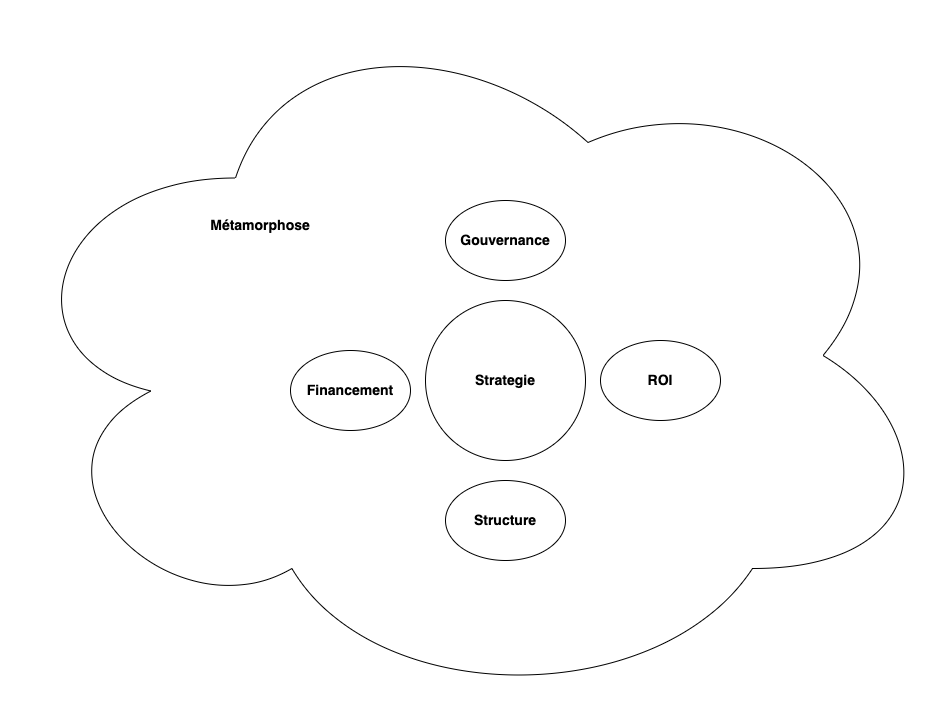
\includegraphics[width=0.7\linewidth]{principes} \end{center}

\hypertarget{la-muxe9tamorphose}{%
\subsection*{La métamorphose}\label{la-muxe9tamorphose}}
\addcontentsline{toc}{subsection}{La métamorphose}

Le paradigme de la métamorphose de l'orienté-service est décrit comme l'aspect le plus important de la modélisation orienté-service.
Le cycle de vie orienté service est centré sur la perspective de développement et d'exploitation d'un service et sur son passage dans le temps au cours de sa durée de vie. Ici, la principale préoccupation est le traitement d'un service lors des événements du cycle de vie. Cela concerne les mécanismes qui ont été commandés pour utiliser une exécution sans faille du service et pour assurer la continuité des activités dans l'environnement de production. La figure ci-dessous illustre les quatre principaux états de transformation du cycle de vie orienté service:

\begin{center}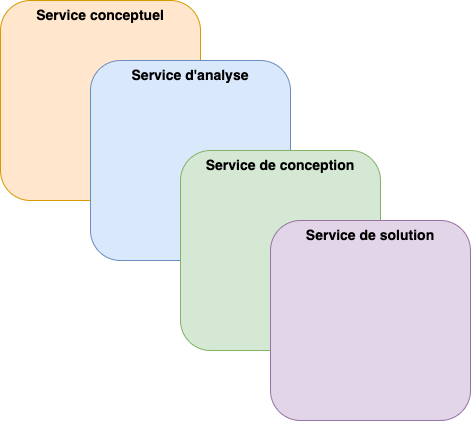
\includegraphics[width=0.7\linewidth]{evolutionservice} \end{center}

Au départ un service apparaît simplement comme une idée et un concept. Plus tard,il devient une unité d'analyse. Lorsque la phase d'analyse est terminée, le service se transforme en une entité de conception. Enfin, le cycle de vie de développement orienté service génère un service de solution physique prêt à être déployé dans des environnements de production.

Chapters and sections are numbered by default. To un-number a heading, add a \texttt{\{.unnumbered\}} or the shorter \texttt{\{-\}} at the end of the heading, like in this section.

\hypertarget{principes-de-duxe9veloppement-des-applications-orientuxe9es-service}{%
\chapter{Principes de développement des applications orientées service}\label{principes-de-duxe9veloppement-des-applications-orientuxe9es-service}}

Cross-references make it easier for your readers to find and link to elements in your book.

\hypertarget{chapters-and-sub-chapters}{%
\section{Chapters and sub-chapters}\label{chapters-and-sub-chapters}}

There are two steps to cross-reference any heading:

\begin{enumerate}
\def\labelenumi{\arabic{enumi}.}
\tightlist
\item
  Label the heading: \texttt{\#\ Hello\ world\ \{\#nice-label\}}.

  \begin{itemize}
  \tightlist
  \item
    Leave the label off if you like the automated heading generated based on your heading title: for example, \texttt{\#\ Hello\ world} = \texttt{\#\ Hello\ world\ \{\#hello-world\}}.
  \item
    To label an un-numbered heading, use: \texttt{\#\ Hello\ world\ \{-\#nice-label\}} or \texttt{\{\#\ Hello\ world\ .unnumbered\}}.
  \end{itemize}
\item
  Next, reference the labeled heading anywhere in the text using \texttt{\textbackslash{}@ref(nice-label)}; for example, please see Chapter \ref{cross}.

  \begin{itemize}
  \tightlist
  \item
    If you prefer text as the link instead of a numbered reference use: \protect\hyperlink{cross}{any text you want can go here}.
  \end{itemize}
\end{enumerate}

\hypertarget{captioned-figures-and-tables}{%
\section{Captioned figures and tables}\label{captioned-figures-and-tables}}

Figures and tables \emph{with captions} can also be cross-referenced from elsewhere in your book using \texttt{\textbackslash{}@ref(fig:chunk-label)} and \texttt{\textbackslash{}@ref(tab:chunk-label)}, respectively.

See Figure \ref{fig:nice-fig}.

\begin{Shaded}
\begin{Highlighting}[]
\FunctionTok{par}\NormalTok{(}\AttributeTok{mar =} \FunctionTok{c}\NormalTok{(}\DecValTok{4}\NormalTok{, }\DecValTok{4}\NormalTok{, .}\DecValTok{1}\NormalTok{, .}\DecValTok{1}\NormalTok{))}
\FunctionTok{plot}\NormalTok{(pressure, }\AttributeTok{type =} \StringTok{\textquotesingle{}b\textquotesingle{}}\NormalTok{, }\AttributeTok{pch =} \DecValTok{19}\NormalTok{)}
\end{Highlighting}
\end{Shaded}

\begin{figure}

{\centering 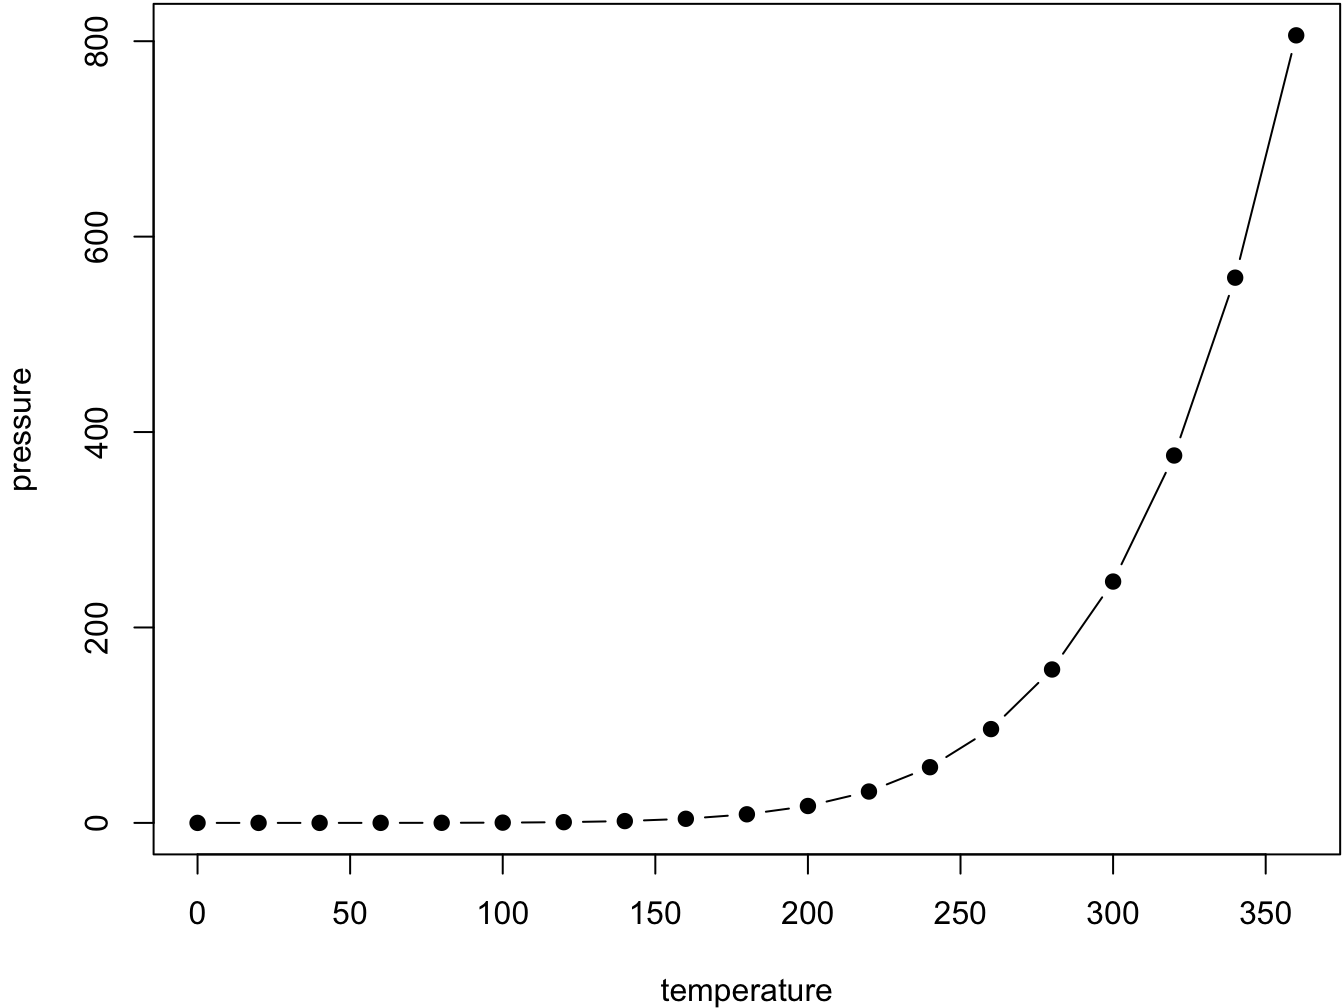
\includegraphics[width=0.8\linewidth]{_main_files/figure-latex/nice-fig-1} 

}

\caption{Here is a nice figure!}\label{fig:nice-fig}
\end{figure}

Don't miss Table \ref{tab:nice-tab}.

\begin{Shaded}
\begin{Highlighting}[]
\NormalTok{knitr}\SpecialCharTok{::}\FunctionTok{kable}\NormalTok{(}
  \FunctionTok{head}\NormalTok{(pressure, }\DecValTok{10}\NormalTok{), }\AttributeTok{caption =} \StringTok{\textquotesingle{}Here is a nice table!\textquotesingle{}}\NormalTok{,}
  \AttributeTok{booktabs =} \ConstantTok{TRUE}
\NormalTok{)}
\end{Highlighting}
\end{Shaded}

\begin{table}

\caption{\label{tab:nice-tab}Here is a nice table!}
\centering
\begin{tabular}[t]{rr}
\toprule
temperature & pressure\\
\midrule
0 & 0.0002\\
20 & 0.0012\\
40 & 0.0060\\
60 & 0.0300\\
80 & 0.0900\\
\addlinespace
100 & 0.2700\\
120 & 0.7500\\
140 & 1.8500\\
160 & 4.2000\\
180 & 8.8000\\
\bottomrule
\end{tabular}
\end{table}

\hypertarget{moduxe8les}{%
\chapter{Modèles}\label{moduxe8les}}

You can add parts to organize one or more book chapters together. Parts can be inserted at the top of an .Rmd file, before the first-level chapter heading in that same file.

Add a numbered part: \texttt{\#\ (PART)\ Act\ one\ \{-\}} (followed by \texttt{\#\ A\ chapter})

Add an unnumbered part: \texttt{\#\ (PART\textbackslash{}*)\ Act\ one\ \{-\}} (followed by \texttt{\#\ A\ chapter})

Add an appendix as a special kind of un-numbered part: \texttt{\#\ (APPENDIX)\ Other\ stuff\ \{-\}} (followed by \texttt{\#\ A\ chapter}). Chapters in an appendix are prepended with letters instead of numbers.

\hypertarget{protocoles-et-normes}{%
\chapter{Protocoles et normes}\label{protocoles-et-normes}}

\hypertarget{footnotes}{%
\section{Footnotes}\label{footnotes}}

Footnotes are put inside the square brackets after a caret \texttt{\^{}{[}{]}}. Like this one \footnote{This is a footnote.}.

\hypertarget{citations}{%
\section{Citations}\label{citations}}

Reference items in your bibliography file(s) using \texttt{@key}.

For example, we are using the \textbf{bookdown} package \citep{R-bookdown} (check out the last code chunk in index.Rmd to see how this citation key was added) in this sample book, which was built on top of R Markdown and \textbf{knitr} \citep{xie2015} (this citation was added manually in an external file book.bib).
Note that the \texttt{.bib} files need to be listed in the index.Rmd with the YAML \texttt{bibliography} key.

The RStudio Visual Markdown Editor can also make it easier to insert citations: \url{https://rstudio.github.io/visual-markdown-editing/\#/citations}

\hypertarget{approche-et-mise-en-oeuvre}{%
\chapter{Approche et mise en oeuvre}\label{approche-et-mise-en-oeuvre}}

\hypertarget{equations}{%
\section{Equations}\label{equations}}

Here is an equation.

\begin{equation} 
  f\left(k\right) = \binom{n}{k} p^k\left(1-p\right)^{n-k}
  \label{eq:binom}
\end{equation}

You may refer to using \texttt{\textbackslash{}@ref(eq:binom)}, like see Equation \eqref{eq:binom}.

\hypertarget{theorems-and-proofs}{%
\section{Theorems and proofs}\label{theorems-and-proofs}}

Labeled theorems can be referenced in text using \texttt{\textbackslash{}@ref(thm:tri)}, for example, check out this smart theorem \ref{thm:tri}.

\begin{theorem}
\protect\hypertarget{thm:tri}{}\label{thm:tri}For a right triangle, if \(c\) denotes the \emph{length} of the hypotenuse
and \(a\) and \(b\) denote the lengths of the \textbf{other} two sides, we have
\[a^2 + b^2 = c^2\]
\end{theorem}

Read more here \url{https://bookdown.org/yihui/bookdown/markdown-extensions-by-bookdown.html}.

\hypertarget{callout-blocks}{%
\section{Callout blocks}\label{callout-blocks}}

The R Markdown Cookbook provides more help on how to use custom blocks to design your own callouts: \url{https://bookdown.org/yihui/rmarkdown-cookbook/custom-blocks.html}

\hypertarget{sharing-your-book}{%
\chapter{Sharing your book}\label{sharing-your-book}}

\hypertarget{publishing}{%
\section{Publishing}\label{publishing}}

HTML books can be published online, see: \url{https://bookdown.org/yihui/bookdown/publishing.html}

\hypertarget{pages}{%
\section{404 pages}\label{pages}}

By default, users will be directed to a 404 page if they try to access a webpage that cannot be found. If you'd like to customize your 404 page instead of using the default, you may add either a \texttt{\_404.Rmd} or \texttt{\_404.md} file to your project root and use code and/or Markdown syntax.

\hypertarget{metadata-for-sharing}{%
\section{Metadata for sharing}\label{metadata-for-sharing}}

Bookdown HTML books will provide HTML metadata for social sharing on platforms like Twitter, Facebook, and LinkedIn, using information you provide in the \texttt{index.Rmd} YAML. To setup, set the \texttt{url} for your book and the path to your \texttt{cover-image} file. Your book's \texttt{title} and \texttt{description} are also used.

This \texttt{gitbook} uses the same social sharing data across all chapters in your book- all links shared will look the same.

Specify your book's source repository on GitHub using the \texttt{edit} key under the configuration options in the \texttt{\_output.yml} file, which allows users to suggest an edit by linking to a chapter's source file.

Read more about the features of this output format here:

\url{https://pkgs.rstudio.com/bookdown/reference/gitbook.html}

Or use:

\begin{Shaded}
\begin{Highlighting}[]
\NormalTok{?bookdown}\SpecialCharTok{::}\NormalTok{gitbook}
\end{Highlighting}
\end{Shaded}


  \bibliography{book.bib,packages.bib}

\end{document}
